\chapter{GAN} 
\section{Motivation} 
Example 1: Great test log-likelihood, poor samples. For a discrete noise mixture models, let $p_\theta(x) = 0.01 p_{data}(x) + 0.99 p_{noise}(x)$
    \begin{align*}
        \log p_\theta(x) 
        & = \log(0.01p_{data}(x) + 0.99p_{noise}(x))\\
        & \geq \log(0.01p_{data}(x))\\
        & = \log p_{data}(x) - \log 100\\
        & \Longrightarrow E_{p_{data}}[\log p_\theta(x)] \geq E_{p_{data}}[\log p_{data}(x)] - \log 100]\\
        & E_{p_{data}}[\log p_\theta(x)] \leq  E_{p_{data}}[\log p_{data}(x)] \tag{By non-negative KL divergence} 
    \end{align*}
As we increase the dimension of $x$, absolute value of $\log p_{data} (x)$ increases proportionally. So eventually we will have high likelihood, but garbage samples. 

\section{Comparing distributions via samples but not likelihood} 
Given $S_1 = \{ x \sim P \}$ and $S_2 = \{ x \sim Q \}$, a two -sample test considers the following hypotheses: 
    \begin{itemize}
        \item Null: $P = Q$
        \item Alternative: $P \neq Q$
    \end{itemize}
A test statistics $T$ is a function of samples, and can be used to compare $s_1, s_2$. Such as means, and variance. \\

\section{Settings} 
We can always assume that $s_1$ is from the data, i.e.: $s_1 =  \{ x \sim p_{data} \}  = \{ x \in D \} $. In addition, our generative model with distribution $p_\theta$ should permits efficient sampling, so we have $s_2 = \{x \sim p_\theta \}$. We use a neural network discriminator to conduct two-sample test. The discriminator will try to maximizes the two-sample test objective. 

\section{GAN Objective} 
Discriminator objective (predict 1 for x sampled from data, predict 0 for x generated from generator): 
    \begin{align*}
        max_{D} V(G,D) = E_{x\sim P_{data}}[\log D(x)] + E_{x\sim P_G}[\log(1-D(X)]
    \end{align*}

Generator objective (generator takes in noise $z$ and maps to $x$):
    \begin{align*}
        min_{G} max_{D}V(G,D) = E_{x\sim P_{data}}[\log D(x)] + E_{x\sim P_G}[\log(1-D(X)]
    \end{align*}
i.e.: Generator objective is to minimize the loss described for discriminator

\section{Jenson-Shannon Divergence} 
JSD is a symmetric version of KL divergence and its squareroot satisfies the triangle inequality. 
    \begin{align*}
        D_{JSD}(p,q) = \frac{1}{2}(D_{KL}(p, \frac{p + q}{2}) + D_{KL}(q, \frac{p+q}{2}))
    \end{align*}
with the optimal discriminator $D_G^*$, we see GAN minimizes a scaled and shifted Jensen-Shannon divergence $ \overset{min}{G} 2D_{JSD}(P_{data}, P_G) - \log 4$

\section{Training GAN}
Sample minibatch of $m$ training points $x^{(1)}, ..., x^{(m)}$ from dataset $D$. Sample minibatch of $m$ noise vector $z^{(1)}, ..., z^{(m)}$ from $p_z$. \\
Update the discriminator parameters $\phi$ by stochastic gradient ascent 
    \begin{align*}
        \nabla_\phi V(G_\theta, D_\phi) = \frac{1}{m} \nabla_\phi \sum_{i=1}^m [\log D_\phi(x^{(i)}) + \log (1 - D_\phi(G_\theta(z^{(i)})))]
    \end{align*}
Update the generator parameters $\theta$ by stochastic gradient descent 
    \begin{align*}
        \nabla_\theta V(G_\theta, D_\phi) = \frac{1}{m} \nabla_\theta \sum_{i=1}^m [\log (1 - D_\phi(G_\theta(z^{(i)})))]
    \end{align*}

\section{f-GAN} 
Given two densities $p$ and $q$, the $f$-divergence is given by 
    \begin{align*}
        D_f(p,q) = E_{x\sim q}[f(\frac{p(x)}{q(x)})]
    \end{align*}
where $f$ is any convex, lower-semicontinuous function with $f(1) = 0$
    \begin{itemize}
        \item Convex: Line joining any two points lies above the function. (Non-negative second derivative)
        \item Lower-semicontinuous: At discontinuous point, function value at any point $x_0$ is close to $f(x_0)$ or greater than $f(x_0)$
        \item By convex and Jensen's inequality: $E_{x\sim q}[f(\frac{p(x)}{q(x)})] \geq f(E_{x\sim q}[\frac{p(x)}{q(x)}]) = f(1) = 0$ i.e.: f-divergence is always non-negative 
    \end{itemize}
In order to use f-divergences as a two-sample test objective for likelihood free learning, we need to be able to estimate it only via samples. \\

Frenchel Conjugate: for any function $f(\cdot)$. its convex conjugate is defined as 
    \begin{align*}
        f*(t) = \sup_{u\in domain_f}(ut 0 f(u))
    \end{align*}
    \begin{itemize}
        \item $f^*$ is always convex and lower semi-continuous 
        \item $f^{**} \leq f$
        \item $f^{**} = f$ when $f(\cdot)$ is convex, lower semicontinuous. Equivalently, $f(u) = f^{**}(u) = sup_{t\in domin_{f^*}} (tu - f^*(t))$
    \end{itemize}
We can obtain a lower bound to any f-divergence via its Fenchel conjugate. Because f-divergence might not necessarily directly computable. 
    \begin{align*}
        D_f(p,q) 
        & = E_{x\sim q}[f(\frac{p(x)}{q(x)})] \tag{Definition of $f$- divergence}\\
        & = E_{x\sim q}[sup_{t\in domain_{f^*}} (t \frac{p(x)}{q(x)} - f^*(t))]\\
        & := E_{x\sim q}[T^*(x) \frac{p(x)}{q(x)} - f^*(T^*(x))] \tag{Let $T^*(x)$ be the optimal t that maximizes the value} \\
        & = \int_X T^*(x) * p(x) - f^*(T^*(x)) q(x) \quad dx \\
        & = sup_T \int_X T(x) * p(x) - f^*(T(x)) q(x) \quad dx \\
        & \geq sup_{T \in \mathcal{T}} \int_X T(x) * p(x) - f^*(T(x)) q(x) \quad dx  \tag{$\mathcal{T}$ is an arbitrary class of function} \\
        & = sup_{T \in \mathcal{T}} E_{x\sim p}[T(x)] - E_{x\sim q}[f^*(T(x))] 
    \end{align*}
Note this lower bound is likelihood-free w.r.t $p$ and $q$ because we can use Monte Carlo to estiamte the expected value. Conceptually, maxing $T$ means to push up the value of $T$ on samples from $p$ (real data) and push down the value for $x$ from $q$ (generator). 


So we can establish f-GAN as :
    \begin{itemize}
        \item Choose any f-divergence 
        \item Let $p = p_{data}$, and $q = p_G$
        \item Parameterize $T$ by $\phi$ and G by $\theta$
        \item The objective is $min_\theta max_\phi F(\theta, \phi) = E_{x\sim p_{data}}[T_\phi(x)] - E_{x\sim p_{G_\theta}}[f^*(T_\phi(x))]$
        \item Generator $G_\theta$ tries to minimize the divergence estimate, and discriminator $T_\phi$ tries to tighten the lower bound
    \end{itemize}
Limitation of f-GAN: 
    \begin{itemize}
        \item The support of $q$ has to cover the support of $p$. Otherwise discontinuity arises in $f-$ divergences
    \end{itemize}

\section{Wasserstein GAN} 
Wasserstein distance is defined as: 
    \begin{align*}
        D_w(p,q) = \inf_{\gamma \in \prod(p,q)} E_{(x,y) \sim \gamma}[ \norm{x-y}_1]
    \end{align*}
Where $\prod(p,q)$ contains all joint distributions of $(x,y)$ where the marginal distribution of $x$ is $p(x)$ and the marginal distribution of $y$ is $q(y)$. $\gamma(y|x)$ is a probabilistic earth moving plan that warps $p(x)$ to $q(y)$. \\

Kantorovich-Rubinstein duality describes the Wasserstein distance in the form of optimization problem. 
    \begin{align*}
        D_w(p,q) = \sup_{\norm{f}_{L\leq 1}} E_{x\sim p}[f(x)] - E_{x\sim q}[f(x)]
    \end{align*}
$\norm{f}_{L\leq 1}$ means that the Lipschitz constant of $f(x)$ is 1. i.e.: 
    \begin{align*}
        \forall x,y: \abs{f(x) - f(y)} \leq \norm{x-y}_1
    \end{align*}
    
So the Wasserstein GAN with discriminator $D_\phi(x)$ and generator $G_\theta(z)$
    \begin{align*}
        \min_\theta \max_\phi E_{x\sim p_{data}}[D_\phi(x)] - E_{z\sim p(z)}[D_\phi(G_\theta(z))]
    \end{align*}
The Lipschitzness of $D_\phi(x)$ is enforced through weight clipping or gradient penalty. 

\section{BiGAN and latent representations} 
BiGAN framework: 
    \begin{figure}[H]
        \centering
        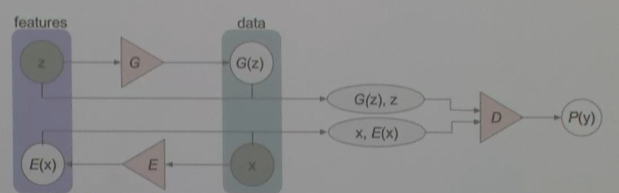
\includegraphics{images/003_BiGAN.png}
    \end{figure}
\begin{itemize}
    \item Encoder network $E$ only observes $x\sim p_{data}(x)$ during training to learn a mapping $E:x \to z$.
    \item The generator network only observes the samples from the prior $z \sim p(z)$ to learn a mapping $G:z\to x$
    \item The discriminator $D$ now observes samples from the generative model $z, G(z)$ and the encoding distribution $E(x), x$, and try to discriminate. 
    \item After training is complete, new samples are generated via $G$ and latent representation encoder $E$
\end{itemize}

\section{Translating across domains} 
Let's say we have distribution $X$ and distribution $Y$. CycleGAN structure: 
    \begin{itemize}
        \item Conditional Generative models $G: X \to Y$
        \item Conditional Generative model $F: Y \to X$
        \item Discriminator $D_y$ compares the observed dataset $Y$ and the generated samples $\hat{Y}=G(X)$
        \item Discriminator $D_x$ compares the observed dataset $X$ and the generated sample $\hat{X} = F(Y)$
        \item Cycle consistency: $F(G(X)) \approx X$ and $G(F(Y)) \approx Y$
    \end{itemize}
The overall loss function is 
    \begin{align*}
        \min_{F,G,D_x,D_y} L_{GAN}(G,D_y,X,Y) + L_{GAN}(F,D_x,X,Y) + \lambda (E_X[\norm{F(G(X)) - X}_1] + E_Y[\norm{G(F(Y))-Y}_1]
    \end{align*}
